\documentclass{beamer}
\usetheme{Antibes} 
\usepackage{textcomp}
\begin{document}
	\title{Mashbot}
	\author{Andrew Gall, Vito Salerno, Josiah Kiehl, G. Nicholas D'Andrea, and Cody Ray}
	\date{\today}

	\frame{\titlepage}
	
	\frame{\frametitle{Table of Contents} \tableofcontents}

	\section{Rationale}
		
		\subsection{Why it is needed?}
			\frame{Why Mashbot?}
		  \frame{\begin{figure}
\includegraphics[width=5cm]{pngs/p1.png}\end{figure}}
		  \frame{\begin{figure}
\includegraphics[width=5cm]{pngs/p2.png}\end{figure}}
		  \frame{\begin{figure}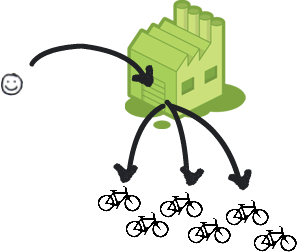
\includegraphics[width=3cm]{pngs/p3.png}\end{figure}}
		  \frame{\begin{figure}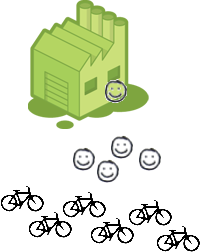
\includegraphics[width=2cm]{pngs/p5.png}\end{figure}}
		  \frame{\begin{figure}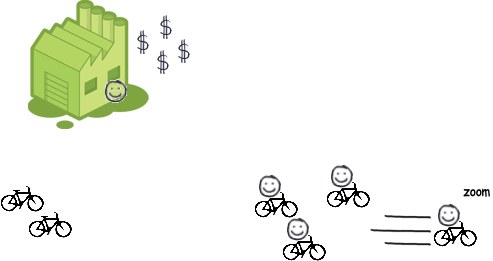
\includegraphics[width=5cm]{pngs/p6.png}\end{figure}}
		  \frame{\begin{figure}
\includegraphics[width=2cm]{pngs/p7.png}\end{figure}}
		  \frame{\begin{figure}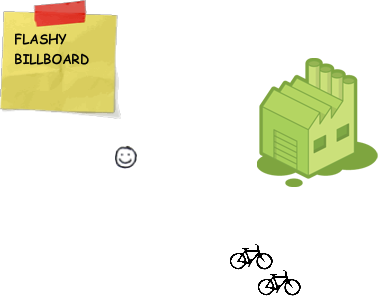
\includegraphics[width=5cm]{pngs/p8.png}\end{figure}}
		  \frame{\begin{figure}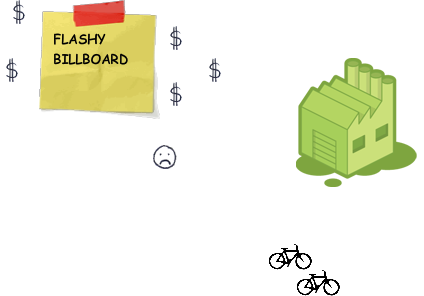
\includegraphics[width=5cm]{pngs/p9.png}\end{figure}}
		  \frame{\begin{figure}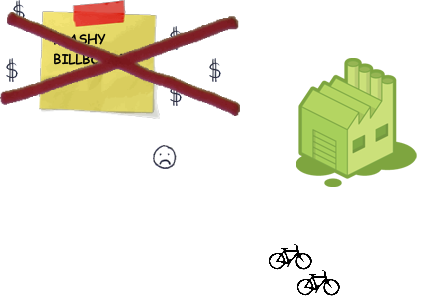
\includegraphics[width=5cm]{pngs/p10.png}\end{figure}}
		  \frame{\begin{figure}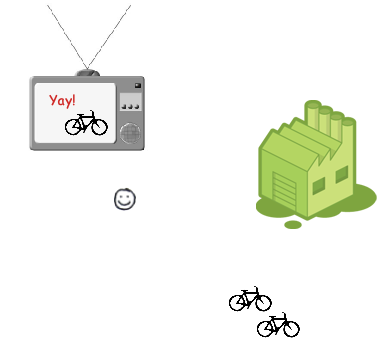
\includegraphics[width=5cm]{pngs/p11.png}\end{figure}}
		  \frame{\begin{figure}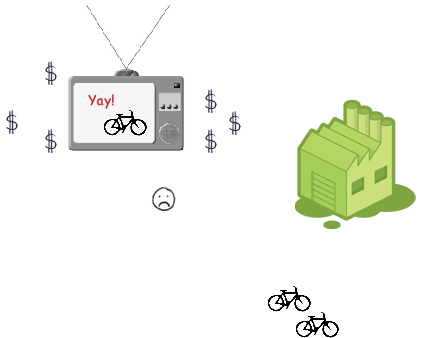
\includegraphics[width=5cm]{pngs/p12.png}\end{figure}}
		  \frame{\begin{figure}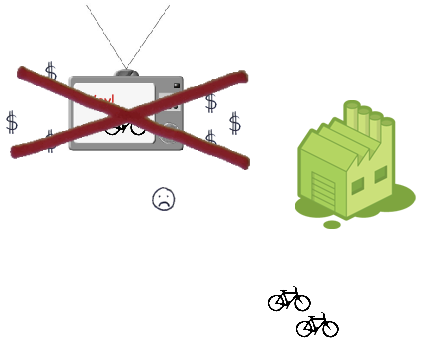
\includegraphics[width=5cm]{pngs/p13.png}\end{figure}}
		  \frame{\begin{figure}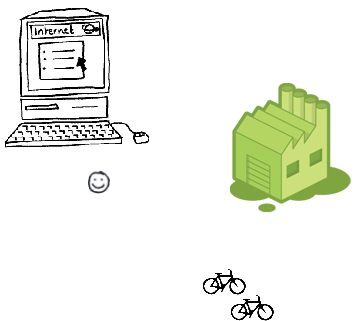
\includegraphics[width=5cm]{pngs/p14.png}\end{figure}}
		  \frame{\begin{figure}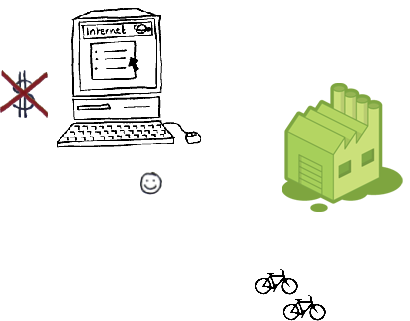
\includegraphics[width=5cm]{pngs/p15.png}\end{figure}}
		  \frame{\begin{figure}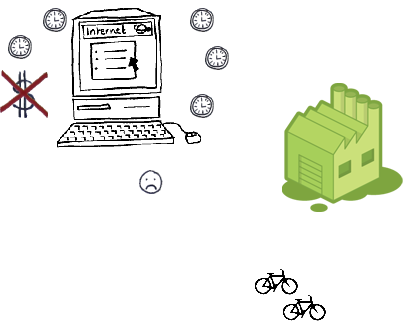
\includegraphics[width=5cm]{pngs/p16.png}\end{figure}}
		  \frame{\begin{figure}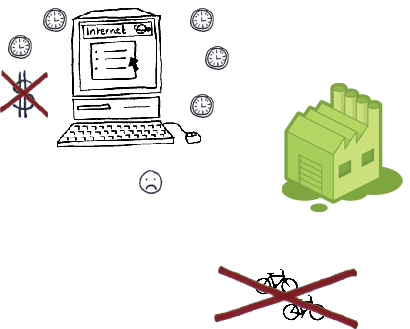
\includegraphics[width=5cm]{pngs/p17.png}\end{figure}}
		  \frame{\begin{figure}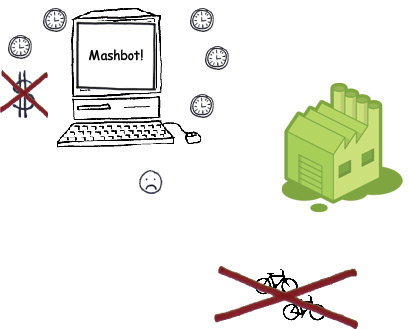
\includegraphics[width=5cm]{pngs/p18.png}\end{figure}}
		  \frame{\begin{figure}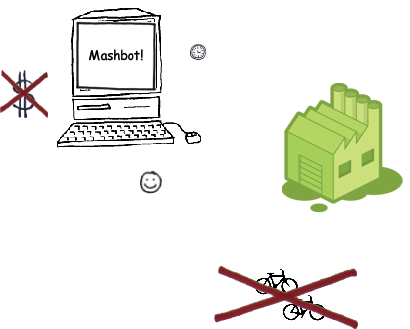
\includegraphics[width=5cm]{pngs/p19.png}\end{figure}}
		  \frame{\begin{figure}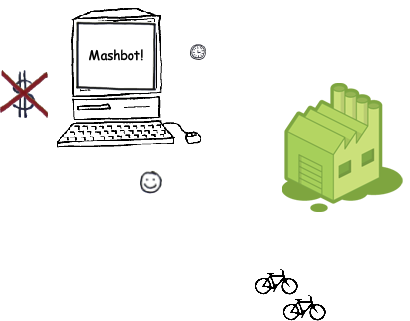
\includegraphics[width=5cm]{pngs/p20.png}\end{figure}}
		  \frame{\begin{figure}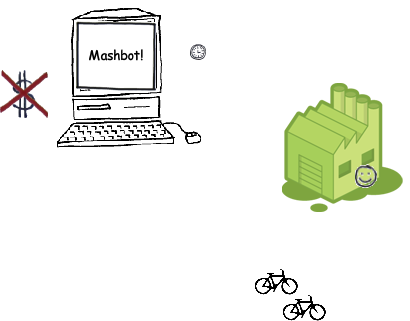
\includegraphics[width=5cm]{pngs/p21.png}\end{figure}}
		  \frame{\begin{figure}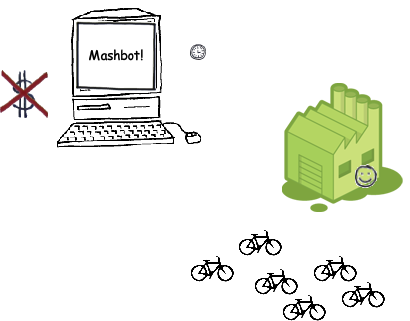
\includegraphics[width=5cm]{pngs/p22.png}\end{figure}}
		  \frame{\begin{figure}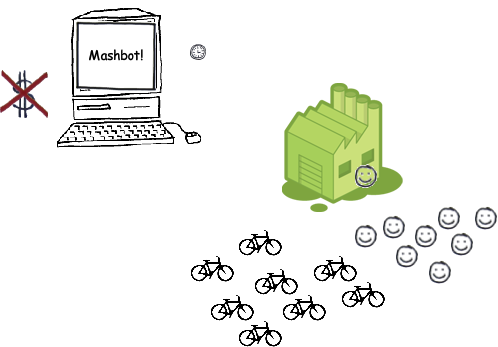
\includegraphics[width=5cm]{pngs/p23.png}\end{figure}}
		  \frame{\begin{figure}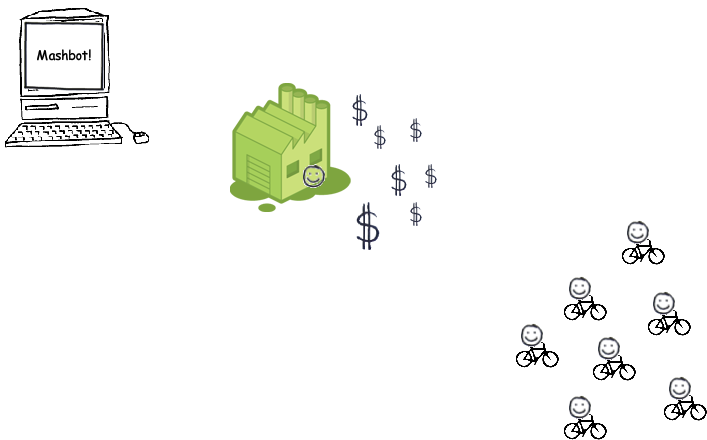
\includegraphics[width=5cm]{pngs/p24.png}\end{figure}}
                  
		\subsection{Who needs Mashbot?}
                \frame{Who needs Mashbot?}
			\frame{\frametitle{Target Customers}
				\begin{itemize}
					\item Small Business Owners
					\item Non-Profits
					\item Authors
				\end{itemize}	
			}
                  \section{Similar Products}
                  
                     \frame{Haven't other people solved this problem?}
			\frame{\frametitle{Salesforce.com}
                          \begin{itemize}
                            \item Pros
                            \begin{itemize}
                               \item Interfaces with Facebook, Twitter
                            \end{itemize}
                            \item Cons
                            \begin{itemize}
                               \item Focused on sales to individual,
                                 mostly established clients
                               \item Is focused on customer service
                                 instead of marketing
                            \end{itemize}
                          \end{itemize}
                        }
			\frame{\frametitle{Mailchimp.com}
                          \begin{itemize}
                            \item Pros
                            \begin{itemize}
                               \item Campaign Statistics
                               \item A\textbackslash B Split Testing
                            \end{itemize}
                            \item Cons
                            \begin{itemize}
                               \item Only does email
                            \end{itemize}
                          \end{itemize}
                        }
                        \frame{\frametitle{Visible Technologies}
                          \begin{itemize}
                            \item Pros
                            \begin{itemize}
                               \item Provides social network monitoring
                               \item Enables engagement in social
                                 networking conversations
                            \end{itemize}
                            \item Cons
                            \begin{itemize}
                               \item Not built for running marketing
                                 campaigns
                               \item They seem to be targeting large
                                 corporations
                            \end{itemize}
                          \end{itemize}
	                }
                        \section{Design}
                        \subsection{Architecture}
                        \frame{Mashbot has a better design}
                        \frame{\frametitle{How Mashbot works}
                          \begin{itemize}
                            \item Website
                            \item Two-tiered architecture
                              \begin{itemize}
                                \item Campaign Manager
                                \item Publishing/Aggregation Platform
                                \item \emph{This decoupling provides reliability 
                                  and flexibility}
                              \end{itemize}
                            \end{itemize}

                        }
                        \frame{\frametitle{Campaign Manager}
                          \begin{itemize}
                            \item Interacts with social networking sites in a 
                              unified way
                            \item Schedules multi-part campaigns and monitors them
                            \item Quick, intuitive interface
                          \end{itemize}
                        }
                        \frame{\frametitle{Publishing/Aggregation Platform}
                          \begin{itemize}
                            \item Plugin oriented
                            \item Push/pull query architecture 
                            \item Allows complex data requests across
different services
                          \end{itemize}
                        }
                        \subsection{User Interface}
                        \frame{\huge{\centering{User Interface}}}
                        \section{Current Status}
                        \frame{\huge{\centering{Prototype}}}
                        \section{Questions\textinterrobang}
                        \frame{\centering{\Large{Questions}\LARGE{\textinterrobang}}}
                        
\end{document}
